\documentclass[10pt, a4paper]{exam}
\printanswers			 % Comment this line to hide the answers 
\usepackage[utf8]{inputenc}
\usepackage[T1]{fontenc}
\usepackage[ngerman]{babel}
\usepackage{listings}
\usepackage{float}
\usepackage{graphicx}
\usepackage{color}
\usepackage{listings}
\usepackage[dvipsnames]{xcolor}
\usepackage{tabularx}
\usepackage{geometry}
\usepackage{color,graphicx,overpic}
\usepackage{amsmath,amsthm,amsfonts,amssymb}
\usepackage{tabularx}
\usepackage{listings}
\usepackage[many]{tcolorbox}
\usepackage{multicol}
\usepackage{hyperref}
\usepackage{pgfplots}
\usepackage{bussproofs}
\usepackage{tikz}
\usetikzlibrary{automata, arrows.meta, positioning}
\renewcommand{\solutiontitle}{\noindent\textbf{Antwort}: }
\SolutionEmphasis{\small}
\geometry{top=1cm,left=1cm,right=1cm,bottom=1cm} 

\pdfinfo{
 /Title (Grundlagen der Biosignalverarbeitung - Prüfungsvorbereitung)
 /Creator (TeX)
 /Producer (pdfTeX 1.40.0)
 /Author (Robert Jeutter)
 /Subject ()
}
\title{Grundlagen der Biosignalverarbeitung - Prüfungsvorbereitung}
\author{}
\date{}

% Don't print section numbers
\setcounter{secnumdepth}{0}

\newtcolorbox{myboxii}[1][]{
 breakable,
 freelance,
 title=#1,
 colback=white,
 colbacktitle=white,
 coltitle=black,
 fonttitle=\bfseries,
 bottomrule=0pt,
 boxrule=0pt,
 colframe=white,
 overlay unbroken and first={
 \draw[red!75!black,line width=3pt]
 ([xshift=5pt]frame.north west) -- 
 (frame.north west) -- 
 (frame.south west);
 \draw[red!75!black,line width=3pt]
 ([xshift=-5pt]frame.north east) -- 
 (frame.north east) -- 
 (frame.south east);
 },
 overlay unbroken app={
 \draw[red!75!black,line width=3pt,line cap=rect]
 (frame.south west) -- 
 ([xshift=5pt]frame.south west);
 \draw[red!75!black,line width=3pt,line cap=rect]
 (frame.south east) -- 
 ([xshift=-5pt]frame.south east);
 },
 overlay middle and last={
 \draw[red!75!black,line width=3pt]
 (frame.north west) -- 
 (frame.south west);
 \draw[red!75!black,line width=3pt]
 (frame.north east) -- 
 (frame.south east);
 },
 overlay last app={
 \draw[red!75!black,line width=3pt,line cap=rect]
 (frame.south west) --
 ([xshift=5pt]frame.south west);
 \draw[red!75!black,line width=3pt,line cap=rect]
 (frame.south east) --
 ([xshift=-5pt]frame.south east);
 },
}

\begin{document}
\begin{myboxii}[Disclaimer]
  Aufgaben aus dieser Vorlage stammen aus der Vorlesung \textit{Grundlagen der Biosignalverarbeitung} und wurden zu Übungszwecken verändert oder anders formuliert! Für die Korrektheit der Lösungen wird keine Gewähr gegeben.
\end{myboxii}

%##########################################
\begin{questions}

  \question Sensoren
  \begin{parts}
    \part Welche Arten von Sensoren existieren?
    \begin{solution}
      \begin{description}
        \item[Aktiv] gibt Spannung/Strom ab, wobei er für Funktion Energie benötigt/umwandelt. wirkt wie elektrische Signalquelle
        \item[Passiv] ändert elektrische Größen (z.B. Widerstand) ohne Energiezufuhr von außen
      \end{description}
    \end{solution}

    \part Wie lösen Sensoren auf? Mit Beispielen
    \begin{solution}
      \begin{description}
        \item[temporal] Zeitabstand zwischen Messungen (z.B. Aktionspotentiale)
        \item[spektral] Abstand von Spektrallinien (z.B. Wärmebildkamera)
        \item[räumlich] räumlicher Abstand (z.B. EEG, Ultraschall)
        \item[...] Kombinationen (z.B. spatialtemporale Auflösung in Frequenzband)
      \end{description}
    \end{solution}

    \part In welche Klassen können Messgrößen unterschieden werden?
    \begin{solution}
      \begin{description}
        \item[Physikalisch] Kraft, Druck, Moment, Durchfluss
        \item[Elektrizität] Potential, Strom, Impedanz
        \item[Magnetismus] Fluss, Induktion
        \item[Optik/Licht] spektrale Dämpfung, Extinktion
        \item[Chemisch] Partialdruck von Gasen, Zucker, Hämoglobin
        \item[Akustik] Herzschalltöne, Atmung
        \item[Temperatur] Körpertemperatur
      \end{description}
    \end{solution}

    \part Welche Methoden sind unter Ultraschall nutzbar?
    \begin{solution}
      \begin{description}
        \item[CW] (Continous Wave) keine Tiefeninformation, Information über Dopplerfrequenz mit hoher Variationsbreite, stochastischer Charakter mit viel Rauschen
        \item[PW] (pulsed Wave) Auflösung von der Signalverarbeitung abhängig, physikalische Grenzen erreicht
        \item[Doppler-Technologie] CW/PW vereint, Summe aller Vor- und Nachteile
      \end{description}
    \end{solution}
  \end{parts}

  \question Übertragung
  \begin{parts}
    \part Warum muss man bei der Übertragung von Biosignale über größere Distanz das Signal modulieren?
    \begin{solution}
      Theoretisch können Signale direkt übertragen werden. Dabei können jedoch Störsignale auf das abgenommene Signal einwirken und dieses verfälschen oder das Signal ist zu schwach und geht bei der Übertragung verloren bzw kommt nicht am Empfänger an.

      Deshalb ist es Empfohlen, das abgenommene Biosignal 1. zu verstärken und 2. gegeüber Störungen resistent zu modulieren.
    \end{solution}

    \part Welche Form der analogen Modulation ist besonders Störungsresistent und warum?
    \begin{solution}
      Eine besonders Störresistente Form der Modulation ist die Analog-Digital-Wandlung des Analogen Signals in sein digitales Äquivalent. Auch mit größeren äußeren Störungen, die auf das digitale Signal einwirken, kann der Empfänger durch die große Differenz zwischen 0- und 1- Signalen klar unterscheiden und das Originalsignal (falls notwendig/gewünscht) rücktransformieren in sein Original.
    \end{solution}
  \end{parts}

  \question Elektroden
  \begin{parts}
    \part Welche chemischen/elektrische Vorgänge an Elektroden
    \begin{solution}
      \begin{itemize}
        \item Metallelektrode umgeben von selektiv durchlässiger Membran eingetaucht in die zu untersuchende Elektrolytlösung
        \item die zur Elektrode gelangenden Ionen (Moleküle) verändern die Potentialdifferenz zwischen Mess- und Bezugselektrode
        \item Spannung proportional log. Ionenkonzentration (pH)
        \item Bsp $pCO_2$-Elektrode: $CO_2+H_2O \Leftrightarrow H_2CO_3 \Leftrightarrow H^+ HCO_3^-$
      \end{itemize}
    \end{solution}

    \part Probleme bei Signalauswertung
    \begin{solution}
      Metallelektroden selbst können polarisierbar sein und positiv geladene Metallionen in der Elektrolytlösung das Signal verfälschen.
    \end{solution}

    \part Elektroden auf Haut erzeugen Gleichspannung. Wie entsteht diese Gleichspannung?
    \begin{solution}
      polarisierbare Metallelektroden $\rightarrow$ positiv geladene Metallionen gelangen in umgebende Elektrolytlösung $\rightarrow$ molekulare Doppelschicht mit hoher Impedanz für Niederfrequenzbereich (Hochpassfilter bei Ableitung evozierter Potentiale)
    \end{solution}

    \part Wie kann man diese Gleichspannung reduzieren?
    \begin{solution}
      unpolarisierbare Metallelektroden nutzen

      Ag/AgCl: Verminderung und Stabilisierung der galvanischen Spannung $\rightarrow$ geringe Übergangsimpedanzen im gesamten Frequenzbereich

      AgCl-Schicht liegt der Ag-Schicht an, positiv geladene Metallionen gelangen in umgebende Elektrolytlösung $\rightarrow$ molekulare Doppelschicht mit hoher Impedanz für Niederfrequenzbereich (Hochpassfilter bei Ableitung evozierter Potentiale)
    \end{solution}
  \end{parts}

  \question Störungen
  \begin{parts}
    \part Welche Arten von Biosignalen existieren?
    \begin{solution}

      \begin{tabular}{c|c|c}
        Signal       & Frequenz [Hz] & Amplitude [mV] \\\hline
        EKG (Herz)   & 0,2-200       & 0,1-10         \\
        EEG (Hirn)   & 0,5-100       & 2-100 $\mu$V   \\
        EMG (Muskel) & 10-10000      & 0,05 -1
      \end{tabular}
    \end{solution}

    \part Welche Arten von Störungen existieren? Mit Erklärungen
    \begin{solution}

      \begin{tabular}{p{5cm}|p{5cm}|p{5cm}}
        periodische Störungen                                                                & transiente Störungen                                         & biologische Störungen                          \\\hline
        geringes Problem, spektrale Filter                                                   & unbekannter, einmaliger, nicht reproduzierbarer Verlauf      & lassen sich nicht abschalten/kaum unterdrücken \\
        NF-magnetische Felder nicht eliminierbar durch Schirmung, erzeugen Differenzspannung & kaum eliminierbar, Signalform unbekannt/nicht reproduzierbar                                                  \\\hline
        NF-elektrische Felder gut beherrschbar, erzeugen Gleichtaktstörungen                 & bestenfalls Detektion möglich, Messdaten nicht korrigierbar                                                   \\\hline
        HF-Felder immer mehr vorhanden (Kommunikation), Abschirmung unwirtschaftlich         &                                                                                                               \\\hline
        Bsp: öffentliche Stromversorgung                                                     & Bsp: Lastschwankungen                                        & Bsp: Muskelbewegung                            \\
      \end{tabular}

    \end{solution}

    \part Entstehung von biologischen Störungen
    \begin{solution}
      Körperfunktionen lassen sich (ohne Beschädigung) nicht abschalten wie z.B. Rechner. Deshalb wirken unterschiedliche Funktionen des Körpers, wie z.B. Atmung oder Herzschlag auf die Messung ein. Diese Störungen können nicht entfernt werden aber möglichst unterdrücken, indem bestimmte Abnahmepfade (z.B. EKG mit Goldberg) genutzt werden. Die Aktivität des Patienten spielt hierbei eine wichtige Rolle.
      \begin{itemize}
        \item Spektral alle Biosignale im selben Band (0-100Hz)
        \item Nichtlineare Verkopplung der Biosignale verhindern Trennung mit herkömmlichen Methoden
        \item Kein Biosignal deterministisch und reproduzierbar
        \item Transiente/aperiodische, instationäre Biosignale nicht qualifizierbar
        \item Trennung kaum möglich, bestenfalls Reduktion/Abschwächung
        \item Problem: funktionelle Verkopplung/Überlagerung im Mensch
      \end{itemize}
    \end{solution}

    \part Methoden zur Eindämmung von Störungen
    \begin{solution}

      \begin{itemize}
        \item Basislinienschwankung: Gute mechanische Elektrodenfixierung verwenden und prüfen, Kontaktcreme zufügen, eventuell Verwendung anderer Elektroden. Ruhigstellung, Entspannung der Muskeln, Anhalten oder Reduzierung der Atmung.
        \item Netzbrummen: Gerät oder Netzkabel aus Patientennähe entfernen, Kontrolle Elektrodenkontakt! Zur Unterdrückung der 50-Hz-Störungen, die in dem Nutzspektrum des QRS-Komplexes liegt, können nur phasenlineare Filter angewendet werden. Dies ist z.B. mit digitalen Notch-Filtern oder mit Kompensationsfiltern zu erzielen.
        \item Biologische Störungen: Ruhigstellung, Entspannung der Muskeln, Anhalten oder Reduzierung der Atmung
      \end{itemize}
    \end{solution}
  \end{parts}

  \question Gradiometer
  \begin{parts}
    \part Was ist ein Gradiometer?
    \begin{solution}
      Ein Gradiometer wertet den Unterschied zwischen zwei Messungen aus. Zum Beispiel kann ein Gradiometer den Grad messen, auf den ein Hügel ansteigt, d.h. die Differenz der Messung von flacher Erde und der Neigung.
    \end{solution}

    \part Aufbau, Funktionsweise?
    \begin{solution}
      Anordnung mehrerer Beschleunigunsmesser, die je nach Bauart zwischen 10 cm und 1 m voneinander entfernt sind. Die Differenz der Ablesungen zweier Beschleunigungsmesser in eine Raumrichtung, dividiert durch ihren Abstand, entspricht der Messung einer Komponente des Gravitationstensors.
    \end{solution}

    \part Warum stört Erdmagnetfeld nicht? Gradiometerprinzip reicht nicht aus für Erklärung
    \begin{solution}
      Das Erdmagnetfeld wirkt in beiden Messsensoren ungefähr gleich (verschwinded geringer Unterschied je nach Entfernung der Sensoren voneinander). Durch die Differenzbildung wird diese Störung in beiden Sensoren mit entfernt.
    \end{solution}
  \end{parts}

  \question EKG
  \begin{parts}
    \part Wie sieht EKG aus? Zeichne
    \begin{solution}

      \begin{center}
        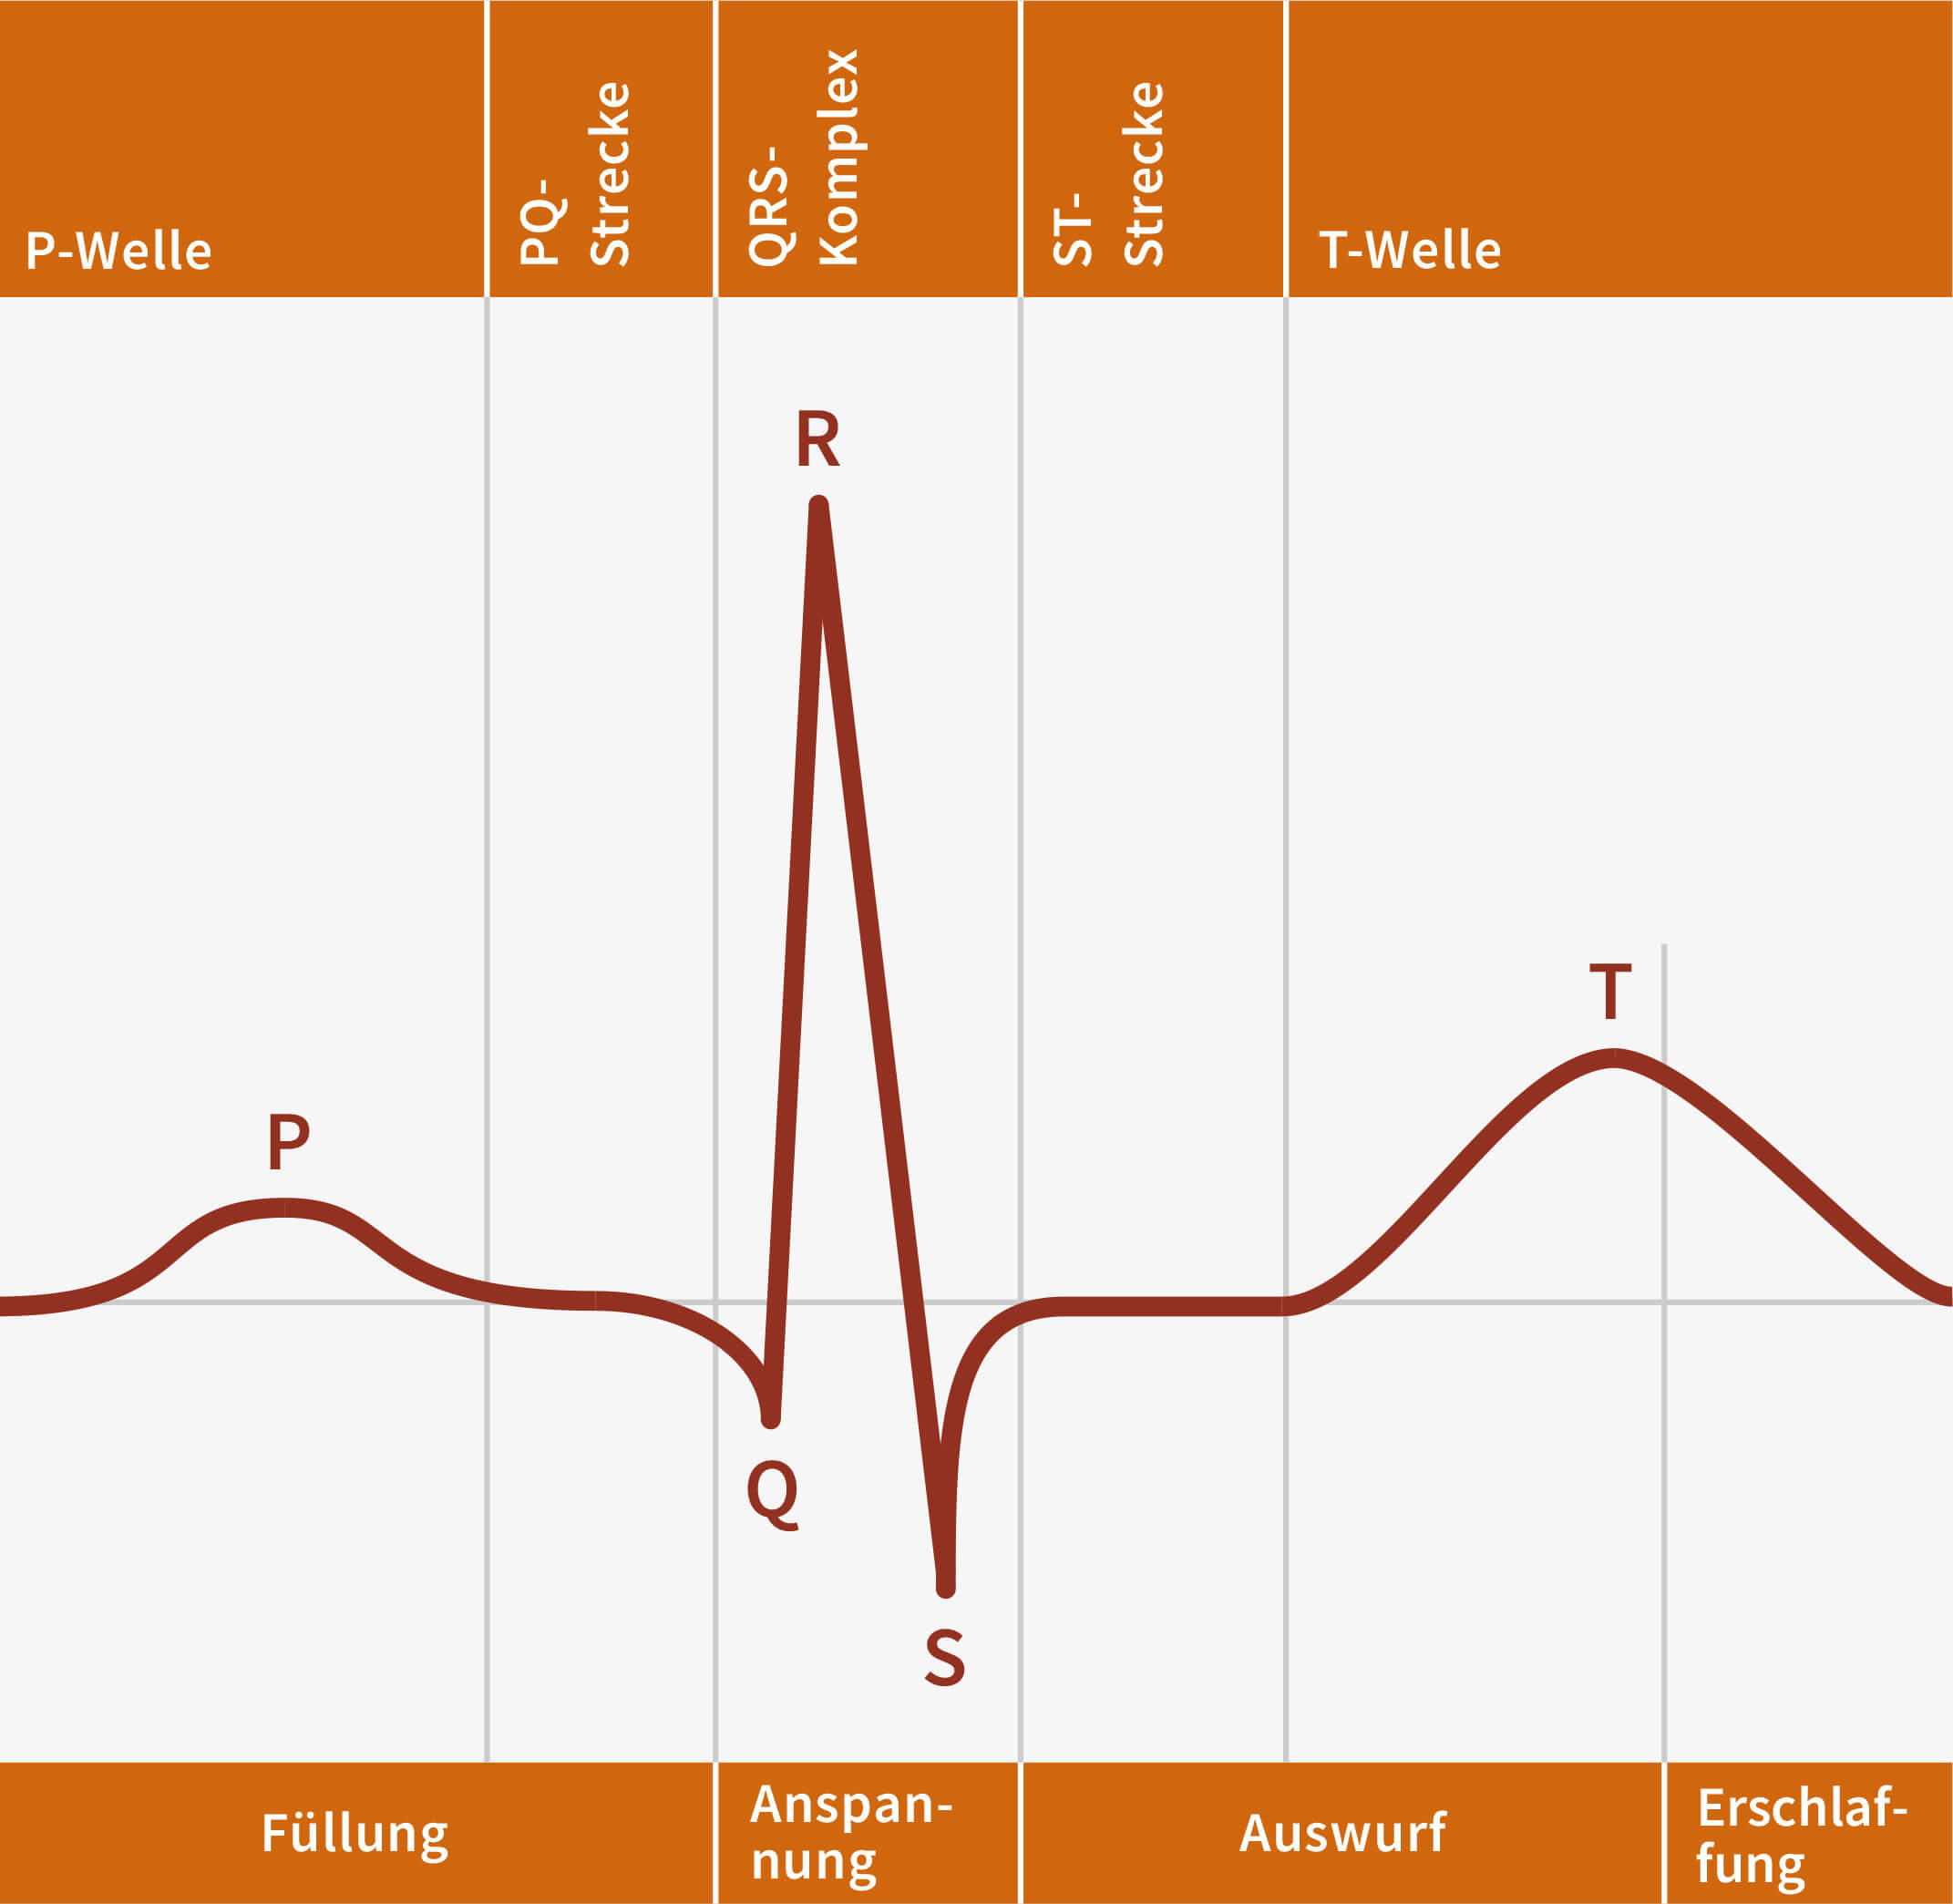
\includegraphics[width=.6\linewidth]{Assets/Biosignalverarbeitung-ekg-verlauf.jpg} %https://www.ratgeber-herzinsuffizienz.de/sites/ratgeber_herzinsuffizienz_de/files/styles/crop_freeform/public/2019-12/ekg-kurve.jpg?itok=2qVKNimN
      \end{center}
    \end{solution}

    \part Was bedeutet welche Zacke?
    \begin{solution}
      \begin{description}
        \item[P-Welle] Füllen der Vorkammern, Erregung in Vorhöfen
        \item[Q.Zacke] Erregnung in Kammern zur Herzspitze
        \item[R-Zacke] Erregung in Kammermuskulatur spitzenwärts
        \item[S-Zacke] Erregnung der Kammerwände breiten sich basalwärts aus
        \item[T-Welle] Erregungsrückgang (umgekehrt registriert)
      \end{description}

      Ablauf
      \begin{enumerate}
        \item Die erschlafften Vorhöfe füllen sich mit Blut.
        \item Beim Zusammenziehen der Vorhöfe strömt das Blut durch die Segelklappen in die Herzkammern.
        \item Während der Anspannungsphase der Kammern schließen sich die Segelklappen.
        \item Beim Zusammenziehen (Systole) drücken die Kammern das Blut durch die geöffneten Taschenklappen in die Hauptschlagader bzw. Lungenschlagader, gleichzeitig beginnen die Vorhöfe sich mit Blut zu füllen.
      \end{enumerate}
    \end{solution}

    \part Arten der Ableitung? Wie und wo abgeleitet?
    \begin{solution}
      \begin{description}
        \item[Bipolare Extremitätenableitung] nach \textbf{Einthoven}
        \item[Unipolare Ableitung] nach \textbf{Wilson} und \textbf{Goldberger} mit Referenz als Sternpunkt der Zusammenschaltung von verschiedene Elektroden über gleich große Widerstände (Durschnittsreferenz)
      \end{description}

      \begin{center}
        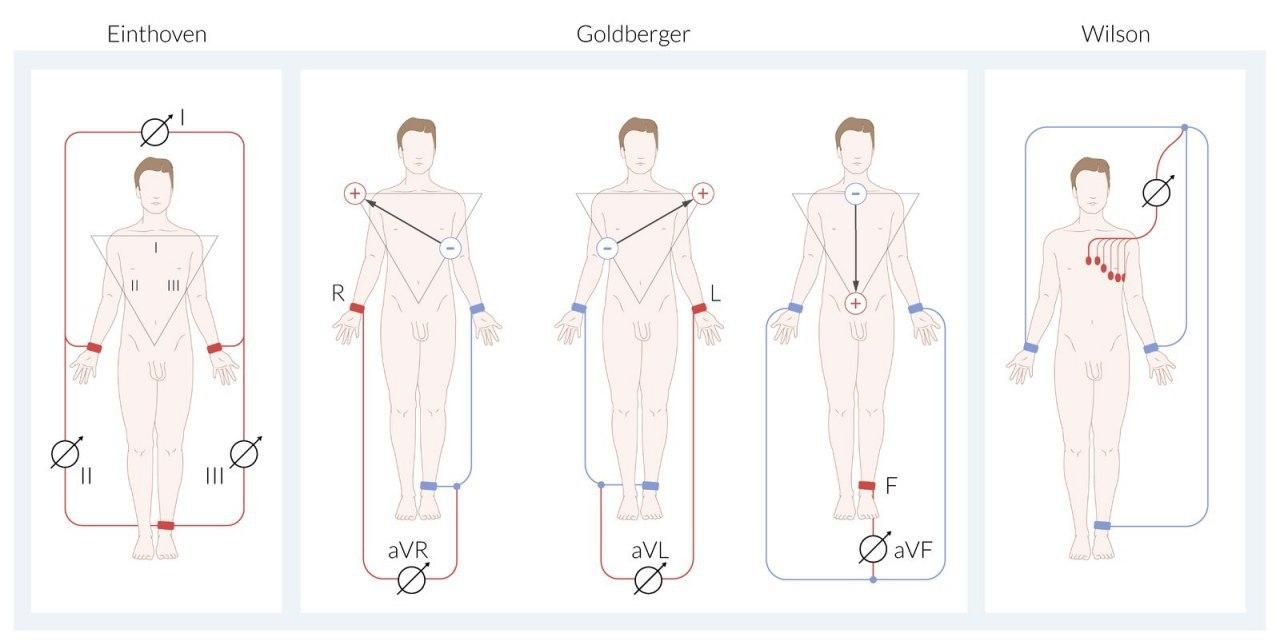
\includegraphics[width=.6\linewidth]{Assets/Biosignalverarbeitung-ekg-ableitung.jpg} %Quelle https://i.pinimg.com/originals/48/d5/f9/48d5f948b3f0f21efad2ad89475dc7b8.jpg
      \end{center}
    \end{solution}

  \end{parts}

  \question EEG
  \begin{parts}
    \part Welche Frequenzbänder?
    \begin{solution}
      \begin{description}
        \item[Delta] 0-4 Hz, Tiefschlaf
        \item[Theta] 4-7 Hz, Schlaf
        \item[Alpha] 8-13 Hz, Wach und in Ruhe
        \item[Beta] 13-30 Hz, Wach mit geistiger Aktivität
        \item[Gamma] $>$30 Hz, starker Konzentration, Lernprozessen oder Meditieren
      \end{description}
    \end{solution}

    \part Nach welchem Prinzip ableiten?
    \begin{solution}
      Da die auf der Kopfhaut zu messenden Signale in der Größenordnung von 5 bis 100 µV liegen, wird ein empfindlicher Messverstärker benötigt. Zur Unterdrückung des allgegenwärtigen Netzbrummens und anderer Störungen wird ein Differenzverstärker mit hoher Gleichtaktunterdrückung benutzt. Aus Gründen der Patientensicherheit ist dieser bei als Medizingerät zugelassenen Elektroenzephalographen als Isolationsverstärker implementiert, wodurch gleichzeitig aber auch die Gleichtaktunterdrückung erhöht wird.

      Die Elektroden für das EEG sind jeweils in einem bestimmten System angebracht, wonach verschiedene Arten von Ableitungen unterschieden werden. Üblich ist das 10-20-System; es werden aber auch alternative Montagen wie das 10-10-System angewendet sowie invasive Ableitungen.
    \end{solution}

    \part Fenster festlegen, wenn Arzt 0,4Hz Auflösung will
    \begin{solution}

      Abtastintervall $T_A$: Zeit zwischen zwei Messpunkten $T_A=\frac{1}{Abtastfrequenz}$

      Zeitfenster: Messzeit $T=N*T_A$ für $N$ Abtast-Punkte

      Niedrigste Frequenz $\Delta f=\frac{1}{N_A * T_A}$

      Höchste Frequenz $f_{max}=\frac{N_A/2}{N_A * T_A}=\frac{1}{2} f_A$
    \end{solution}
  \end{parts}

  \question Guarding-Technik beschreiben
  \begin{solution}
    Schirm am Ausgang eines OV und über Ausgangswiderstand des OV mit der Masse niederohmig verbunden.
    Gleichtaktwiderstand bleibt erhalten, Schutz gegen Störungseinkopplung

    Für Mess-Sicherheit: um Kabel und Guarding-Schirm zweiter Schirm mit Masse verbunden

    $\Rightarrow$ Abschirmung der Signalleitungen vor Störungen aus dem Messkreis
  \end{solution}

  \question Abtasttheorem
  \begin{parts}
    \part Beschreibe
    \begin{solution}
      ein bandbreitenbegrenztes Signal der Grenzfrequenz $f_g$ ist durch seinen periodischen Abtastwert $s(nT)$ vollständig bestimmt, wenn die Abtastrate größer als die Nyquistrate ist: $F_T=\frac{1}{T} > 2*f_G$
    \end{solution}
    \part Abtasttheorem: Welche notwendige und hinreichende Bedingung benötigt man für die Abtastung bei fc=100Hz und USB 0,1...1kHz
    \begin{solution}

    \end{solution}
  \end{parts}

  \question Aliasing erklären
  \begin{solution}
    Frequenzsignale innerhalb der Signalverarbeitung überschritten oder in unzureichender Abtastrate gemessen $\rightarrow$ Verzerrung

    Anti-Aliasing-Filter: wandeln Frequenzen oberhalb der Nyquistfrequenz um und verhindern bei Abtastfrequenz, dass Signale in Frequenz nicht verändert werden
  \end{solution}

  \question Gibbsche Phänomen erklären
  \begin{solution}
    das typische Verhalten von Fourierreihen in der Umgebung von Sprungsstellen. Wird eine Fourierreihe aus einer Funktion mit Unstetigkeiten entwickelt, ergeben sich an den Unstetigkeitsstellen typische Über- und Unterschwinger, die sich aber mit steigendem Anteil hochfrequenter Schwingungen verringern. Erst bei einer unendlichen Reihe verschwinden die Überschwinger.
  \end{solution}

  \question Messverstärker
  \begin{parts}
    \part Welcher Phasenfrequenzgang bei Messverstärker?
    \begin{solution}

    \end{solution}

    \part Warum? Was passiert bei Nichteinhaltung?
    \begin{solution}

    \end{solution}

    \part Eigenrauschen qualitativ beschreiben, aus welchen Komponenten besteht es
    \begin{solution}

    \end{solution}
  \end{parts}

  \question Signal mit $f(t)=2*cos(t*2*\pi *f)$, die Frequenz war 9Hz, das Signal war im Bereich von 0 bis 4,5s gegeben. Gegeben TM,...?
  \begin{parts}
    \part Eine Matlab funktion nutzt $f=fs:df:fe$ um das Fenster zu berechnen. Berechne $fs,df$ und $fe$
    \begin{solution}
      Um Signalfrequenz $f_c$ mit einer der diskreten Frequenzen im DFT-Spektrum zu treffen, muss die Signalfrequenz $f_c$ ein ganzzahliges Vielfaches der spektralen Auflösung $\delta f$ sein: $f_c=\frac{1}{T_c=k*\Delta f=\frac{k}{T_{DFT}}}$. Die Analysezeit $T_{DFT}$ sollte ebenso ganzes vielfaches der Periodendauer $T_C$ sein: $T_{DFT}=k*T_C=N*T_A$

    \end{solution}

    \part Welcher Effekt verursacht viele Spektralteile?
    \begin{solution}
      Leckeffekt: Signal wird in Blöcken verarbeitet, diese Blöcke sind endlich $\rightarrow$ Leckeffekt entsteht, wenn Blocklänge nicht natürlichzahliges Vielfaches der Periode des Signals ist.
      Leckeffekt führt zu Verzerrungen und falsch detektierte Spektraleanteilen durch Überlagerung unterschiedlicher Perioden

    \end{solution}

    \part Welche Eigenschaft muss eine Fensterfunktion haben damit dieser Effekt verringert wird?
    \begin{solution}
      Fenster verhindern Leckeffekt: Signal an Fenster Anfang/Ende ein/ausblenden $\rightarrow$ künstliche Periodisierung


      Varianten: Rechteck-, Dreieck-, Gauß-Fenster
    \end{solution}

    \part Wie muss man die Eigenschaft der Fensterfunktion wählen, damit 1. Dynamischer Amplitudengang und 2. Gute Auflösung im Spektralbereich entsteht?
    \begin{solution}
      \begin{description}
        \item[schmale Fensterung] flache Übergänge, große Sperrdämpfung
        \item[breite Fensterung] steile Übergänge, geringe Sperrdämpfung
      \end{description}
    \end{solution}
  \end{parts}

  \question Filter
  \begin{parts}
    \part Anhand welcher Merkmale kann man einen Filter klassifizieren, ob er FIR oder IIR ist?
    \begin{solution}

      \begin{tabular}{p{7cm}|p{7cm}}
        FIR = Finite Impulse Response                                                          & IIR = Infinite Impulse Response                                             \\\hline
        + Lineare Phase, keine Phasenverzerrung, alle Frequenzen um gleichen Betrag verschoben & + Niedrige Kosten, weniger Koeffizienten + Speicher                         \\
        + Stabil, keine Rückkopplung, niemals instabil                                         & Niedrige Latenzzeit für Echtzeitsteuerung und schnelle HF Anwendung         \\
        + arbiträrer Frequenzgang $\rightarrow$ beliebiger Betragsverlauf                      & + Analoges Äquivalent zur Nachahmung der Eigenschaften von analogen Filtern \\
                                                                                               & + hohe Flankensteilheit                                                     \\
        - hoher Rechen+Speicherbedarf, viel mehr Koeffizienten als IIR                         & - nicht linearer Phaseneigenschaft, besonders an Grenzfrequenzen            \\
        - höhere Latenz: möglicherweise große Gruppenverzögerung                               & - aufgrund Rückkopplung numerisch weniger stabil als FIR                    \\
        - kein analoges Äquivalent                                                             &                                                                             \\
        $y(n)=\sum^{N-1}_{k=0} h(k)x(n-k)$                                                     & $y(n)=\sum^{\infty}_{k=0} h(k) x(n-k)$
      \end{tabular}
    \end{solution}

    \part Können FIR instabil werden? Begründen Sie Ihre Vermutung.
    \begin{solution}
      Nein, keine Rückkopplungen im Filter
    \end{solution}

    \part Wie kann man schnell die Koeffizienten eines FIR Filters ausrechnen?
    \begin{solution}

    \end{solution}
  \end{parts}

  \question Filtertypen (nicht für Informatiker)
  \begin{parts}
    \part Filtertypen anhand ihres Amplitudengangs klassifizieren
    \part Welcher ist am besten für (vorgegebene) Biosignale geeignet und warum?
    \part Filtertypen die nach Namen ihres Erfinders heißen?
    \begin{solution}

      \begin{tabular}{p{3cm}|p{3cm}|p{3cm}|p{3cm}}
        Filter               & Eigenschaften                                                                                                      & Vorteile                                                                                                                              & Nachteile                                                    \\\hline
        Butterworth-Filter   & Maximal flacher Verlauf des Betragsfrequenzganges im Durchlassbereich, Dämpfung im Sperrbereich monoton verlaufend & Gutes Amplitudenverhalten im Durchlass- und Sperrbereich                                                                              & Geringe Flankensteilheit im Übergangsbereich                 \\
        Tschebyscheff-Filter & Welligkeit (Ripple) im Durchlassbereich, Dämpfung im Sperrbereich monoton verlaufend                               & Gute Flankensteilheit im Durchlassbereich                                                                                             & Große Änderung der Gruppenlaufzeit, schlechtes Zeitverhalten \\
        Bessel-Filter        & Impulsformung                                                                                                      & Konstante Gruppenlaufzeit (=lineare Phase) im Durchlassbereich                                                                        & Geringe Flankensteilheit im Übergangsbereich                 \\
        Gauß-Filter          & Impulsformung                                                                                                      & Konstante Gruppenlaufzeit im Durchlass- und Sperrbereich. Kein Überschwingen bei der Sprungantwort. Reduzierte Intersymbolinterferenz & Geringe Flankensteilheit im Übergangsbereich
      \end{tabular}
    \end{solution}
  \end{parts}

  \question Adaptive Noise Cancelller
  \begin{parts}
    \part Erläutern Sie anhand eines Blockschaltbilds die Funktionsweise eines adaptiven noise Cancellers
    \begin{solution}

      \begin{center}
        \includegraphics[width=.6\linewidth]{Assets/biosignalverarbeitung-adaptive-noise-cancellation-system.png}
      \end{center}
    \end{solution}

    \part Was muss für das Rauschen gelten, damit das LMS Prinzip angewendet werden kann? Welche Signale müssen korellieren und welche dürfen nicht in Korrelationsbeziehung stehen?
    \begin{solution}

    \end{solution}

  \end{parts}


  \question LTI System
  \begin{parts}
    \part Blockschaltbild -> daraus die Übertragungsfunktion ableiten,
    \begin{solution}

    \end{solution}

    \part Z-Transformation,
    \begin{solution}

    \end{solution}

    \part Stabilität $y(n)=x(n)+2x(n-1)-3(n-1)$?
    \begin{solution}

    \end{solution}
  \end{parts}

  \question cos Funktion
  \begin{parts}
    \part cos-Fkt. gegeben (Gleichung, Graph zu Original-Fkt. + ihrer DFT), Sample-Freq. 10Hz, Abtastung für 2sec:
    \begin{solution}

    \end{solution}

    \part Matlab-Befehl ermitteln für Parameter der $DFT(f_s, d_f, f_e)$
    \begin{solution}

    \end{solution}

    \part Warum im DFT-Graph soviele Freq-Anteile?
    (vmtl. Leck-Effekt)
    \begin{solution}

    \end{solution}

    \part Ursachen dieses Effekts im Zeit~ und Freq-Bereich (Zeit: Signal nicht genau an Periodengrenze abgeschnitten)
    \begin{solution}

    \end{solution}

    \part Wie durch Fensterung beheben?
    \begin{solution}

    \end{solution}

    \part Wie muss Spektrum des Fenster beschaffen sein um:
    \begin{itemize}
      \item hohe spektrale Auflösung
      \item hohe Amplitudendynamik
    \end{itemize}
    zu erreichen?
    \begin{solution}

    \end{solution}
  \end{parts}

  \question Berechne mit $t_{ab}=10s$, $f_{s1}=9kHz$ und $f_{s2}=10kHz$, peaks gegeben
  \begin{parts}
    \part Abtasttheorem
    \begin{solution}

    \end{solution}

    \part Welche Frequenzbereiche der Signale
    \begin{solution}

    \end{solution}

    \part Fehler - Aliasing, graphisch erklären, wie vermeiden?
    \begin{solution}

    \end{solution}

    \part wie sieht analoges Signal im Spektrum aus?
    \begin{solution}

    \end{solution}
  \end{parts}

  \question Signalflussgraph
  \begin{parts}
    \part Zeitdiskretes vs. Analog?
    \begin{solution}

    \end{solution}

    \part Rekursionsgleichung aus Signalflussgraph ermitteln
    \begin{solution}

    \end{solution}

    \part Übertragungsfunktion Gz(Z) im z-Bereich?
    \begin{solution}

    \end{solution}

    \part Ermitteln aller Pol und Nullstellen
    \begin{solution}

    \end{solution}

    \part Zeichne Pol-Nullstellendiagramm mit b=1
    \begin{solution}

    \end{solution}

    \part Welcher Filtertyp? IIR oder FIR
    \begin{solution}

    \end{solution}

    \part Ist das System stabil? Begründe
    \begin{solution}

    \end{solution}

    \part wie muss man b wählen, damit aus dem System ein Allpass wird (mit b>1)?
    \begin{solution}

    \end{solution}
  \end{parts}

  \question Blockschaltbild
  \begin{parts}
    \part rekursive Gleichung aus Blockschaltbild bestimmen,
    \begin{solution}

    \end{solution}

    \part Übertragungsfunktion ermitteln
    \begin{solution}

    \end{solution}

    \part Pol~/Nullstellen bestimmen
    \begin{solution}

    \end{solution}

    \part Pol~/Nullstellen-Diagramm zeichnen
    \begin{solution}

    \end{solution}

    \part für welchen Parameter a wird aus rekursiver Gleichung ein FIR-Filter?
    \begin{solution}

    \end{solution}

    \part in welchem Intervall für a wird Filter stabil, wann/warum instabil?
    \begin{solution}

    \end{solution}

    \part Eingangssignal als Graph gegeben, Ausgangssignal als Graph bestimmen (Faltung durchführen)
    \begin{solution}

    \end{solution}
  \end{parts}

  \question $H(z)=\frac{1-0,8z^{-1}}{1+0,3z^{-1}}$
  \begin{parts}
    \part Signalflussdiagram zeichnen
    \begin{solution}

    \end{solution}

    \part IIR oder FIR?
    \begin{solution}

    \end{solution}

    \part Differenzgleichung?
    \begin{solution}

    \end{solution}

    \part Pol/Nullstellendiagramm zeichnen?
    \begin{solution}

    \end{solution}

    \part Stabilität im Z- und Zeitbereich?
    \begin{solution}

    \end{solution}
  \end{parts}

\end{questions}
\end{document}